% Copyright (c) 2008-2009 solvethis
% Copyright (c) 2010-2011 Casper Ti. Vector
% Public domain.

\chapter{性能测试与评估}
本章将对支持物理层WiFi安全研究的验证平台GRTSEC进行评估。
首先在\ref{sec:envaluation_env_setup}节介绍测试环境,介绍开发板型号、开发套件版本号等,
其次在\ref{sec:envaluation_performance}节对验证平台的性能进行测试,
然后在\ref{sec:envaluation_demo}节对第五章提出的使用样例进行测试,
最后在\ref{sec:envaluation_summary}节对本章进行总结。

  \section{测试环境}\label{sec:envaluation_env_setup}
  在第四章我们介绍了GRTSEC的前期工作GRT2.0的组成部分,GRTSEC与GRT2.0的组成部分相同,但具体测试环境略有不同。
  在GRTSEC中,我们使用的上位主机是一台支持USB3.0接口、运行有Ubuntu14.04操作系统的计算机,
  FPGA是一块Xilinx VC707板卡\cite{xilinxvc707},
  配置计算机是任意一台支持Xilinx Vivado开发套件的计算机,Windows系统或Linux系统均可,
  射频前端是Analog Device公司的EVAL-AD-FMCOMMS3-EBZ开发板\cite{fmcomms3}。
  FPGA开发工具我们使用的是Xilinx Vivado 2015.2,FPGA嵌入式软件开发工具是Xilinx SDK 2015.2。

  \section{平台性能测试}\label{sec:envaluation_performance}
  在本节我们介绍GRTSEC的性能,GRT2.0的性能可参考\cite{cjh16grt},如吞吐率、延迟等,
  本文主要对GRTSEC相对于GRT2.0的扩展性能进行测试。

  首先是FPGA的资源占用率,GRT2.0的资源占有率见表\ref{tab:envaluate_grt2.0_resource},
  增加GRTSEC的扩展后,资源占用率见表\ref{tab:envaluate_grtsec_resource}。
    \begin{table}[!hbp]
    \centering
    \caption{GRT2.0在VC707开发板上的资源占用率}
    \label{tab:envaluate_grt2.0_resource}
      \begin{tabular}{|l|l|l|l|} \hline
      资源 & 已使用 & 总数 & 占用率 \\ \hline
      Flip-Flop & 76781 & 607200 & 12.65 \\ \hline
      LUT & 98657 & 303600 & 32.50 \\ \hline
      Memory LUT & 4551 & 130800 & 3.48 \\ \hline
      I/O & 224 & 700 & 32.00 \\ \hline
      BRAM & 319 & 1030 & 30.97 \\ \hline
      DSP48 & 294 & 2800 & 10.50 \\ \hline
      BUFG & 17 & 32 & 53.12 \\ \hline
      MMCM & 4 & 14 & 28.57 \\ \hline
      PLL & 1 & 14 & 7.14 \\ \hline
      \end{tabular}
    \end{table}
    \begin{table}[!hbp]
    \centering
    \caption{GRTSEC在VC707开发板上的资源占用率}
    \label{tab:envaluate_grtsec_resource}
      \begin{tabular}{|l|l|l|l|} \hline
      资源 & 已使用 & 总数 & 占用率 \% \\ \hline
      Flip-Flop & 79564 & 607200 & 13.10 \\ \hline
      LUT & 95761 & 303600 & 31.54 \\ \hline
      Memory LUT & 4058 & 130800 & 3.10 \\ \hline
      I/O & 224 & 700 & 32.00 \\ \hline
      BRAM & 263 & 1030 & 25.53 \\ \hline
      DSP48 & 303 & 2800 & 10.82 \\ \hline
      BUFG & 14 & 32 & 43.75 \\ \hline
      MMCM & 4 & 14 & 28.57 \\ \hline
      PLL & 1 & 14 & 7.14 \\ \hline
      \end{tabular}
    \end{table}

  我们可以看到,资源使用率没有增加太多,因为GRTSEC主要利用原有信号进行物理层信息的提取,
  而且采用多级寄存器缓存技术进行帧对齐,而不是用FIFO进行缓存,节约了存储空间。

  然后是嵌入式软件代码的性能,主要体现在传输延迟上。从收到一帧到回复ACK的时间间隔,是最关键的延迟指标,
  如果延迟太高,会大大影响传输性能,留给用户可编程的空间会降低。
  GRTSEC相对GRT2.0增加了读取物理层信息的过程,本节对GRT2.0和GRTSEC在这方面的性能进行对比,
  性能结果见表\ref{tab:envaluate_grtsec_latency}。
  (此处需要搭建两台GRT,互相收发数据测试延迟)
  \begin{table}[!hbp]
  \centering
  \caption{GRTSEC与GRT2.0的延迟性能对比表}
  \label{tab:envaluate_grtsec_latency}
    \begin{tabular}{|l|l|l|l|} \hline
    帧长度 & 调制方式 & GRT2.0延迟 & GRTSEC延迟 \\ \hline
    20 & ?? & ?? & ?? \\ \hline
    100 & ?? & ?? & ?? \\ \hline
    1500 & ?? & ?? & ?? \\ \hline
    4095 & ?? & ?? & ?? \\ \hline
    \end{tabular}
  \end{table}

  我们可以看到,延迟没有增加太多,因为经过精心设计的硬件逻辑,可以保证在软件读取之前将物理层信息准备好。

  最后是读取物理层信息的有效性,选用真实的802.11设备进行测试,地点是北京大学理科五号楼五楼。
  我们在2.4GHz频段的最常用1号信道以及5GHz频段的149信道,对该频段挑选最活跃3个真实设备的进行监听,
  记录频偏、CSI、RSSI、调制方式等物理层信息,绘制成以下图表。

  (此处共7张图,频偏、CSI、RSSI各附上两张图,2.4GHz和5GHz,调制方式附上一张图。
  频偏的图是设备频偏变化图,横轴是时间,纵轴是频偏,画3条线。
  CSI的图是三维的,X轴是时间,Z轴是CSI大小,Y轴是子信道,画3个曲面。
  RSSI与频偏类似。调制方式是分布折线图,6个设备放在一张图里,横轴是调制方式,纵轴是所占比例。)

  我们可以看到,频偏值随时间的变化不大,随设备的变化大,CSI和RSSI随时间变化大。

  \section{样例测试}\label{sec:envaluation_demo}
  在本节对第五章提出的使用样例进行测试。
    \subsection{搭建伪装AP}
    搭建伪装AP主要测试其有效性。
    如图\ref{fig:envaluation_fake_ap}所示,我们利用GRTSEC搭建伪装AP,可以被一部手机连接,手机任意输入一个网址可以跳转到钓鱼页面。
    (下图要换掉,用GRT搭建,修改个SSID,重新截图)
  		\begin{figure}[H]
  			\centering
  			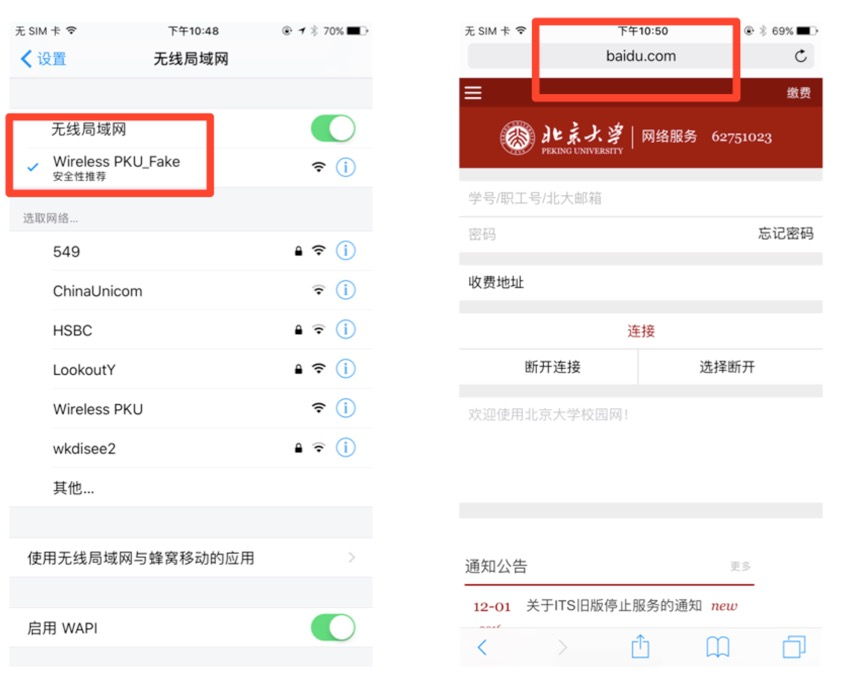
\includegraphics[width=0.5\textwidth]{img/WirelessPKU_fake_1.jpg}
  			\caption{伪装AP与钓鱼认证网页}
  			\label{fig:envaluation_fake_ap}
  		\end{figure}

    我们可以看到,用户手机真实连上了GRTSEC搭建的伪装AP,说明GRTSEC可与商用设备实时通信,
    用户手机看到了钓鱼认证网页,说明GRTSEC兼容上层网络应用。

    \subsection{利用物理层信息识别不同WiFi设备}
    \ref{sec:demo_phy_auth}中提到,我们对三种情况进行测试,区别不同的STA、区别不同地点的AP、区别同一地点的不同AP。

    首先是区别不同的STA,我们对三台设备进行监听,记录频偏值,采用KNN算法,
    测试结果如表\ref{tab:envaluate_identify_sta}所示。
      \begin{table}[!hbp]
      \centering
      \caption{利用物理层信息识别不同的STA}
      \label{tab:envaluate_identify_sta}
        \begin{tabular}{|l|l|l|l|l|} \hline
        设备 & 训练集组数 & 测试集组数 & 正确率 & 误判率 \\ \hline
        华为手机 & ?? & ?? & ?? & ?? \\ \hline
        OPPO手机 & ?? & ?? & ?? & ?? \\ \hline
        三星笔记本电脑 & ?? & ?? & ?? & ?? \\ \hline
        \end{tabular}
      \end{table}

    然后是区别不同的AP,我们对三个WirelessPKU的AP进行监听,以频偏值和时钟偏移为特征进行训练和测试,
    测试结果如表\ref{tab:envaluate_identify_ap}所示。
      \begin{table}[!hbp]
      \centering
      \caption{利用物理层信息识别不同地点的AP}
      \label{tab:envaluate_identify_ap}
        \begin{tabular}{|l|l|l|l|l|} \hline
        设备 & 训练集组数 & 测试集组数 & 正确率 & 误判率 \\ \hline
        WirelessPKU AP1 & ?? & ?? & ?? & ?? \\ \hline
        WirelessPKU AP2 & ?? & ?? & ?? & ?? \\ \hline
        WirelessPKU AP3 & ?? & ?? & ?? & ?? \\ \hline
        \end{tabular}
      \end{table}

    以上两个实验可以看到,通过物理层信息频偏和时钟偏移对不同设备进行识别,正确率较高,
    这种方法可以在多种场景下进行应用。

  \section{总结}\label{sec:envaluation_summary}
  本章对支持物理层WiFi安全研究的验证平台GRTSEC进行了评估,实验表明GRTSEC在没有明显资源占用和性能降低的情况下,
  支持多种物理层信息的提取,通过使用样例说明了支持物理层WiFi安全研究。
